\documentclass[]{../template/Report}%方括号内写yuxi即生成预习报告\documentclass[yuxi]{../template/Report}
\settemplatedir{../template/}%设置模板路径
\usepackage{enumitem}

% Prevent hyperref `Token not allowed in a PDF string' warnings by
% providing safe replacements for math-related tokens in PDF strings.
\AtBeginDocument{%
  \ifdefined\pdfstringdefDisableCommands
	\pdfstringdefDisableCommands{%
	  \def\({}%
	  \def\){}%
	  \def\$ {}%
	  \def\_{}%
	  \def\textsubscript#1{#1}%
	  \def\textsuperscript#1{#1}%
	  \def\ensuremath#1{#1}%
	}%
  \fi
}

\exname{弗兰克赫兹实验} %实验名称
\extable{} %实验桌号
\instructor{} %指导教师
\class{} %班级
\name{} %姓名
\stuid{} %学号

\nyear{} %年
\nmonth{} %月
\nday{} %日
\nweekday{} %星期几,e.g. \nweekday{三}
\daypart{}%上午/下午

\redate{} %如有实验补做,补做日期
\resitu{} %情况说明:

\begin{document}
\maketitle%输出封面

\section{预习报告(10分)}
\subsection{实验综述(5分)}

\subsubsection{实验原理}
\paragraph{波尔原子模型}
\begin{itemize}
\item \textbf{定态假设}:电子在原子中仅能沿特定轨道运动,且不辐射电磁波。这些稳定状态称为“定态”,其中能量最低的E₁为基态,E₂、E₃……为激发态。
\item \textbf{轨道与能量量子化假设}:电子在不同轨道的能量是分立的,不允许处于轨道之间的能量状态。
\item \textbf{跃迁与频率定则}:电子在不同定态间跃迁时,会吸收或发射频率为$\nu$的电磁波,并满足关系:
\begin{equation}
	h\nu = E_m - E_n \quad (h = 6.63 \times 10^{-34} \, \text{J·s})
\end{equation}
\end{itemize}

\paragraph{弗兰克-赫兹管原理}
原子通常处于基态。当受到电磁波或与能量足够的粒子碰撞时,可吸收能量跃迁至激发态。从基态到第一激发态所需能量称为临界能量。
弗兰克-赫兹管内部由阴极K,栅极G1、G2,和板极A组成,如图\ref{fig:弗兰克-赫兹管原理}所示。电子从阴极发出,经电压$U_G2K$加速,在KG2区间与氩原子碰撞,最终到达板极形成电流$I_A$。
实验中,电子在真空中被加速电压$V$加速,获得能量$eV$。若:
\begin{itemize}
\item $eV < E_2 - E_1$:电子与氩原子仅发生弹性碰撞,无能量转移;
\item $eV \geq E_2 - E_1$:发生非弹性碰撞,氩原子吸收$E_2 - E_1$的能量跃迁至激发态,剩余能量仍归电子所有。
\end{itemize}

设激发原子所需电位差为$U_0$,则:
\begin{equation}
	eU_0 = E_2 - E_1
\end{equation}
$U_0$即为氩原子的第一激发电位。实验通过测量板极电流$I_A$随加速电压$U_{G2K}$变化的曲线来测定$U_0$,如图\ref{fig:弗兰克-赫兹管原理}所示。该曲线呈现一系列周期性的波峰与波谷,相邻波峰对应的电压间隔即为$U_0$的测量值。

\begin{figure}[H]
\centering
\begin{minipage}[b]{0.40\textwidth}
	\centering
	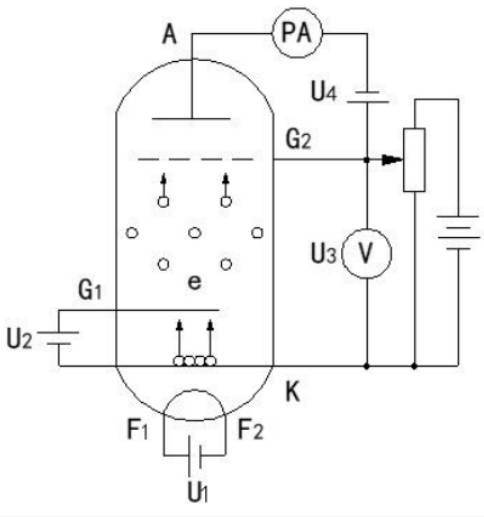
\includegraphics[width=\textwidth]{弗兰克赫兹管.jpg}
\end{minipage}\hfill
\begin{minipage}[b]{0.40\textwidth}
	\centering
	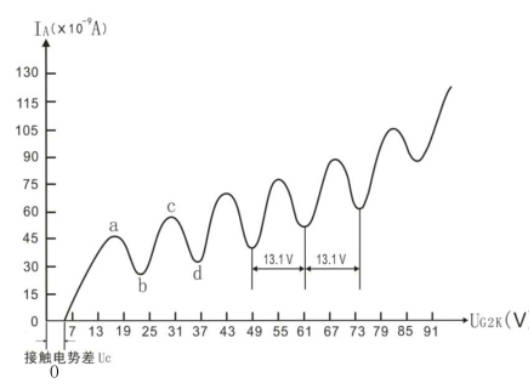
\includegraphics[width=\textwidth]{弗兰克赫兹管1.jpg}
\end{minipage}
\caption{弗兰克-赫兹管原理}
\label{fig:弗兰克-赫兹管原理}
\end{figure}
\subsubsection{实验方法}
实验装置如图所示:
\begin{figure}[H]
\centering
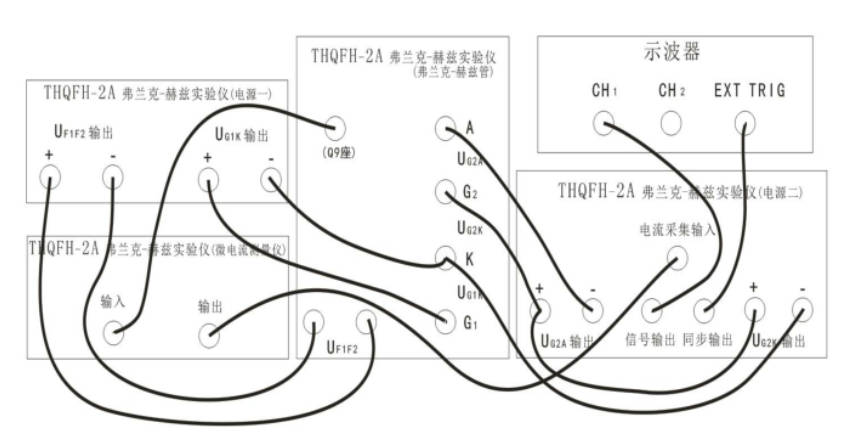
\includegraphics[width=0.6\textwidth]{实验装置示意图.jpg}
\caption{实验装置示意图}
\label{fig:实验装置示意图}
\end{figure}
\paragraph{测量氩原子的第一激发电势(自动测量)}
\begin{enumerate}
\item 正确连接THQFH-2A弗兰克一赫兹实验仪(电源一)、THQFH-2A弗兰克一赫兹实验仪(电源2)、弗兰克赫兹管、微电流测量仪等设备,检查接线。
\item 设置示波器:CH1通道为200mV/div,时间基准为500μs/div;触发类型设为边沿触发,触发源为外部输入,触发类型为下降沿触发,触发模式为自动。
\item 确认“电源二”处于自动测量模式,按下“确认”键启动测量,在示波器上观察$I_A$–$U_{G2K}$曲线的形成过程。
\item 约4分钟后测量结束,记录$U_{G2K}$与$I_A$的7个峰值数据。
\item 重复测量5次,取平均值后使用逐差法计算$U_0$,并估算不确定度。
\end{enumerate}

\paragraph{测量$I_A$–$U_{G2K}$曲线(手动测量)}
\begin{enumerate}
\item 将仪器设为手动测量模式(手动指示灯亮)。
\item 缓慢调节$U_{G2K}$电位器,每间隔0.5V记录一次$I_A$值。电流稳定约4秒后读数。在峰、谷值附近可适当增加测量点以提高精度。
\item 使用软件拟合$I_A$–$U_{G2K}$曲线,判断峰值电压并推算$U_0$。
\end{enumerate}

\subsection{实验重点}
\begin{enumerate}
\item 掌握原子碰撞激发与测量的基本方法。
\item 准确测量氩原子的第一激发电势。
\item 通过实验验证原子能级的存在,深入理解“量子化”概念。
\end{enumerate}

\subsection{实验难点}
本实验难点主要在于仪器的使用:
\begin{enumerate}
\item \textbf{电源与接地}:实验仪与示波器均使用220V/50Hz交流电,必须确保外壳和电源接地可靠。
\item \textbf{参数控制}:需严格按仪器参数设置进行实验,以保证数据有效性。
\item \textbf{预热与调零}:实验前弗兰克-赫兹管需预热20分钟;每次测量前应进行仪器调零。
\item \textbf{量程与保护}:
\begin{itemize}
\item 若微电流显示超量程,应切换较大量程或适当降低灯丝电压$U_{F1F2}$;
\item 若电流剧增,可能为管子击穿,应立即降低$U_{G2K}$与$U_{F1F2}$。
\end{itemize}
\item \textbf{使用时间}:弗兰克-赫兹管单次连续使用不宜超过2小时。
\item \textbf{操作与维护}:搬动仪器需轻拿轻放;实验结束后及时断电,整理导线归位。
\end{enumerate}
\begin{fullreportonly}
\section{原始数据(20分)}

\begin{figure}[H]
    \centering
    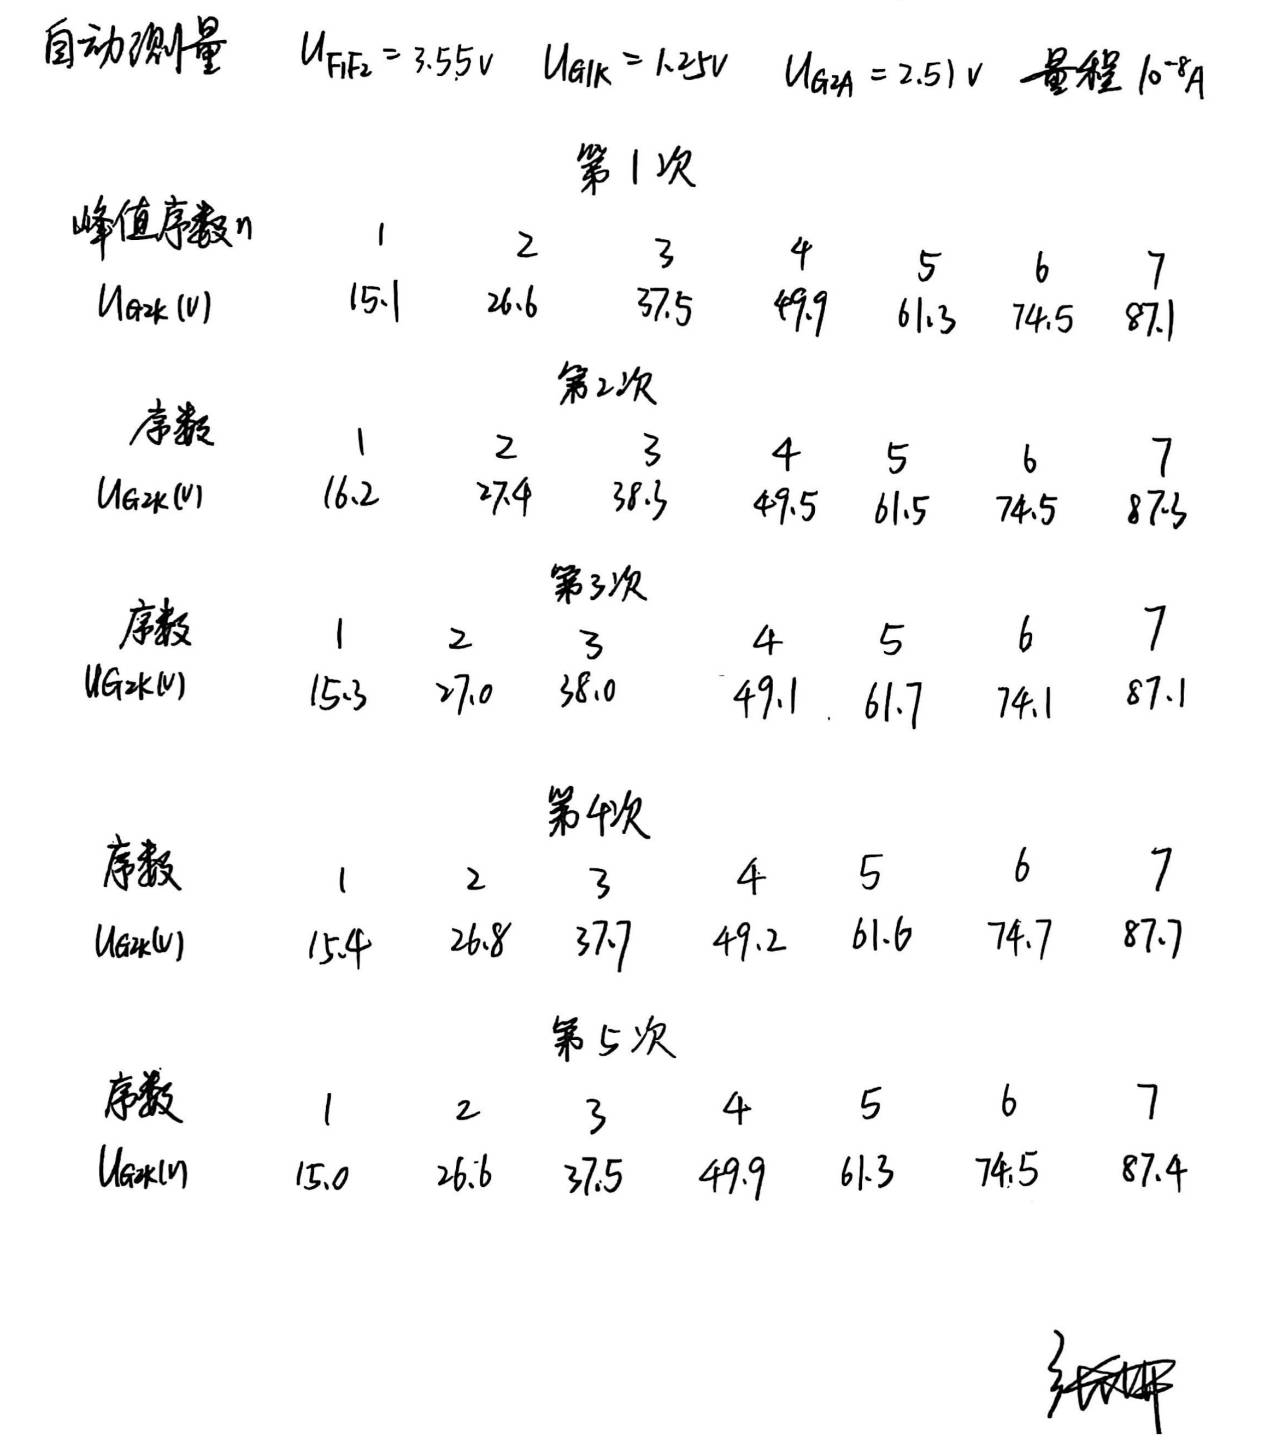
\includegraphics[width=0.6\textwidth]{原始数据1.jpg}
    \caption{自动测量原始数据}
    \label{fig:原始数据记录}
\end{figure}
\begin{figure}[H]
\centering
\begin{minipage}[b]{0.48\textwidth}
	\centering
	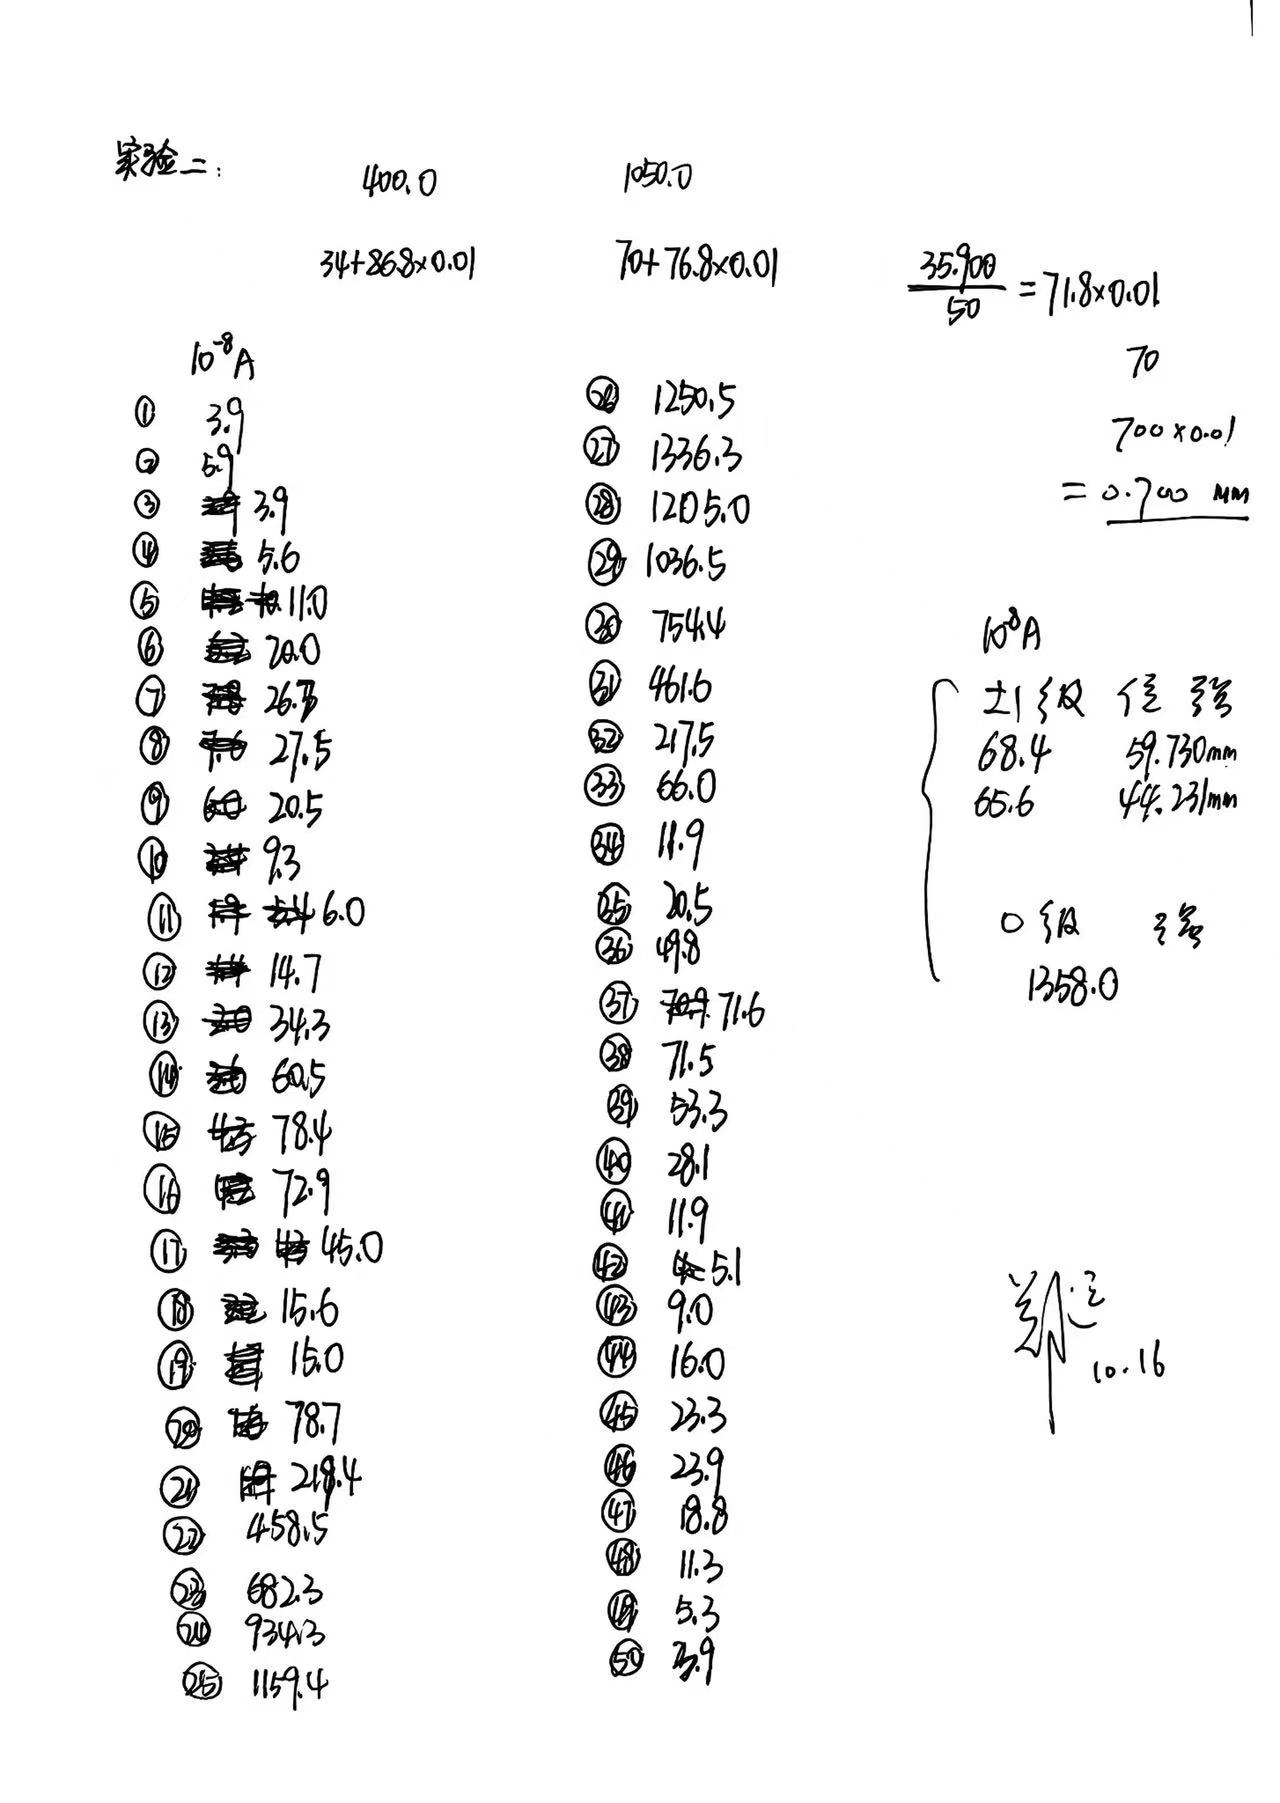
\includegraphics[width=\textwidth]{原始数据2.jpg}
\end{minipage}\hfill
\begin{minipage}[b]{0.48\textwidth}
	\centering
	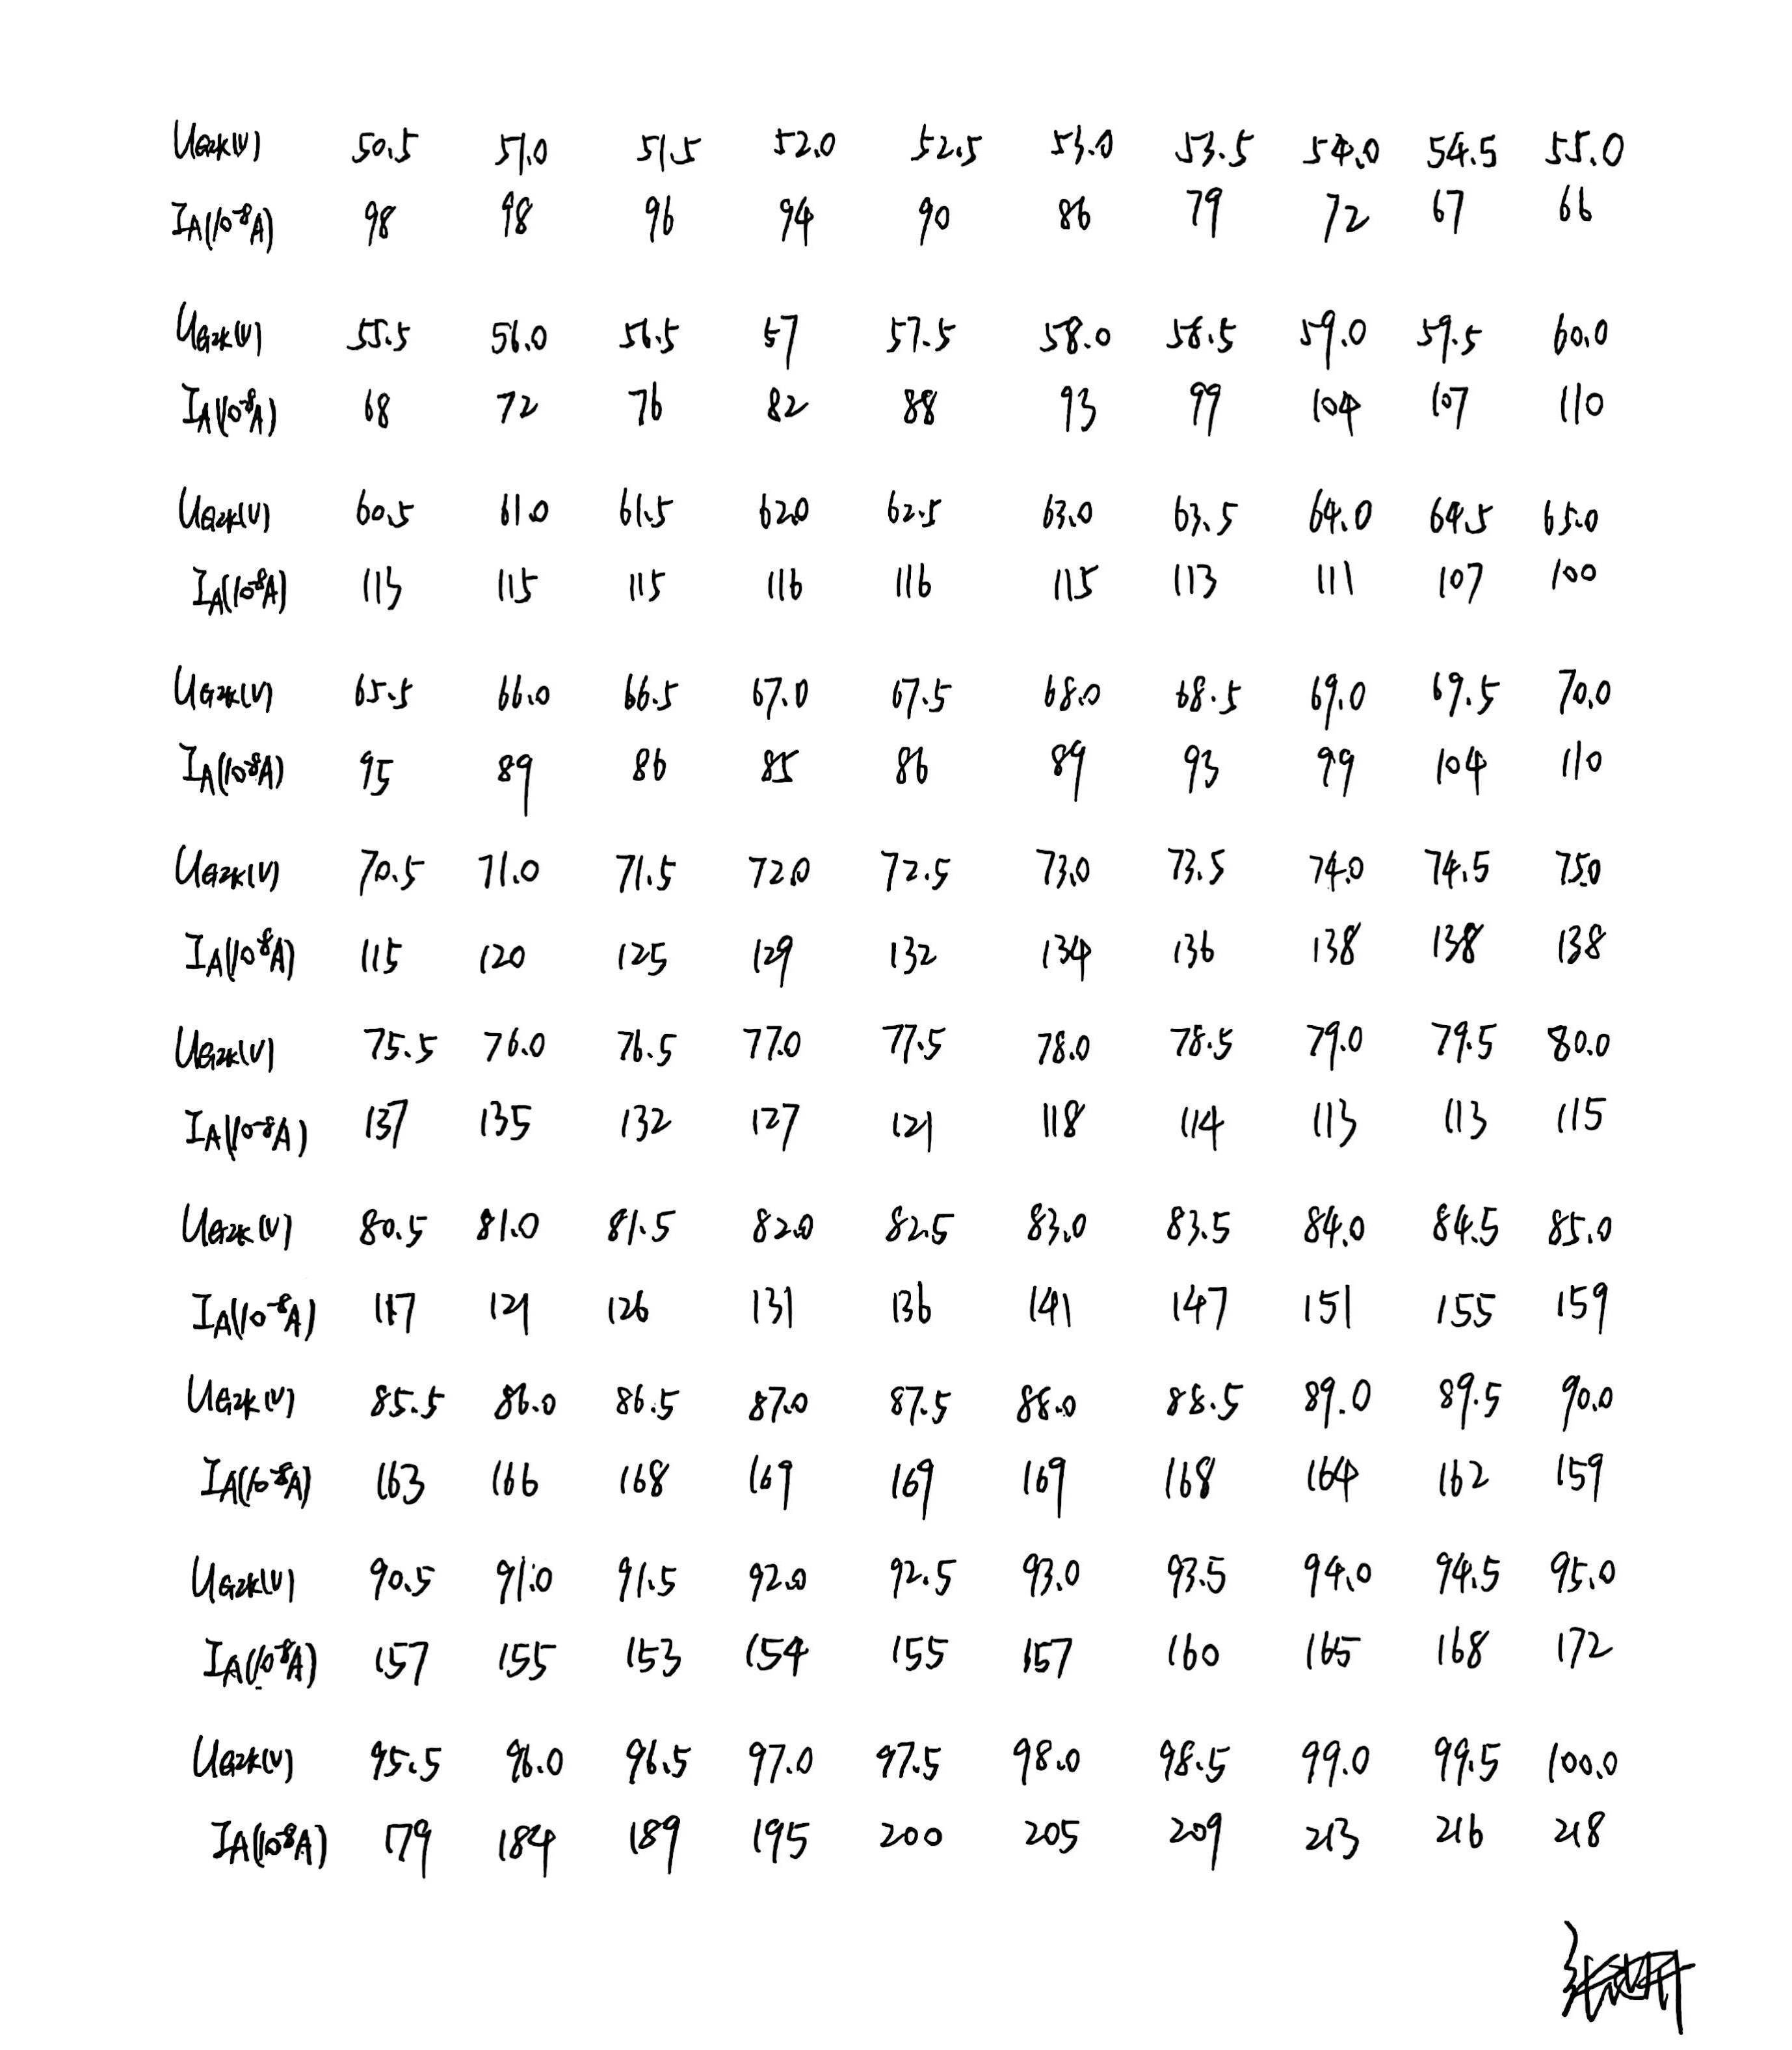
\includegraphics[width=\textwidth]{原始数据3.jpg}
\end{minipage}
\caption{手动测量原始数据}
\label{fig:手动测量原始数据}
\end{figure}
\section{结果与分析(60分)}
\subsection{数据处理与结果(30分)}

\subsubsection{自动测量数据记录与处理}
仪器参数:$U_{F1F2}=4.50V$,$U_{G1K}=1.25V$,$U_{G2A}=3.00V$
\par
微电流测量仪量程选择:$\times 10^{-8}A$
\begin{table}[H]
\centering
\caption{自动测量数据记录表} % 可选:添加表格标题
\label{tab:measurements}
\begin{tabular}{|c|c|c|c|c|c|c|c|}
\hline
\multicolumn{8}{|c|}{\textbf{第 1 次自动测量}} \\
\hline
峰值序号 n & 1 & 2 & 3 & 4 & 5 & 6 & 7 \\
\hline
$U_{G2K}$ (V) & 15.1&26.6 &37.5 &49.9 &61.3 &74.5 &87.1 \\
\hline
\multicolumn{8}{|c|}{\textbf{第 2 次自动测量}} \\
\hline
峰值序号 n & 1 & 2 & 3 & 4 & 5 & 6 & 7 \\
\hline
$U_{G2K}$ (V) &16.2 &27.4 &38.3 &49.5 &61.5 &74.5 &87.3 \\
\hline
\multicolumn{8}{|c|}{\textbf{第 3 次自动测量}} \\
\hline
峰值序号 n & 1 & 2 & 3 & 4 & 5 & 6 & 7 \\
\hline
$U_{G2K}$ (V) &15.3 &27.0 &38.0 &49.1 &61.7 &74.1 &87.1 \\
\hline
\multicolumn{8}{|c|}{\textbf{第 4 次自动测量}} \\
\hline
峰值序号 n & 1 & 2 & 3 & 4 & 5 & 6 & 7 \\
\hline
$U_{G2K}$ (V) &15.4 &26.8 &37.7 &49.2 &61.6 &74.7 &87.7 \\
\hline
\multicolumn{8}{|c|}{\textbf{第 5 次自动测量}} \\
\hline
峰值序号 n & 1 & 2 & 3 & 4 & 5 & 6 & 7 \\
\hline
$U_{G2K}$ (V) &15.0 &26.6 &37.5 &49.9 &61.3 &74.5 &87.4 \\
\hline
\end{tabular}
\end{table}

在弗兰克-赫兹实验中,相邻峰值间隔理论上等于第一激发电势 $U_0$。为减小误差,采用逐差法处理7个峰值电压 $U_1, U_2, \dots, U_7$,计算公式为:
\[
U_0 = \frac{1}{4} \cdot \frac{(U_5 - U_1) + (U_6 - U_2) + (U_7 - U_3)}{3}
\]

代入第一次测量得到的数据,得:
\begin{align*}
U_0^{(1)} = \frac{1}{4} \cdot \frac{(61.3 - 15.1) + (74.5 - 26.6) + (87.1 - 37.5)}{3} = \SI{11.975}{\volt}
\end{align*}
同理可得第2-5次测量结果
\begin{align*}
U_0^{(2)} &= \SI{11.783}{\volt} \\
U_0^{(3)} &= \SI{11.883}{\volt} \\
U_0^{(4)} &= \SI{12.008}{\volt} \\
U_0^{(5)} &= \SI{12.008}{\volt}
\end{align*}
因此,平均第一激发电势为:
\[
\bar{U}_0 = \frac{11.975 + 11.783 + 11.883 + 12.008 + 12.008}{5} = \SI{11.931}{\volt}
\]

已知氩原子第一激发电势理论值为 $U_{\text{理}} = \SI{11.6}{\volt}$,求得相对误差为:
\begin{align*}
\delta = \left| \frac{\bar{U}_0 - U_{\text{理}}}{U_{\text{理}}} \right| \times 100\% = \left| \frac{11.931 - 11.6}{11.6} \right| \times 100\%= \SI{2.85}{\percent}
\end{align*}

根据仪器说明书,第二栅压 $U_{G2K}$ 输出范围为 0--100 V,精度为 $\pm 1\%$,故其绝对误差限为:
\[
\Delta U = 100 \times 1\% = \SI{1.0}{\volt}
\]

假设误差服从均匀分布,则B类标准不确定度为:
\[
u_B(U_{G2K}) = \frac{\Delta U}{\sqrt{3}} = \frac{1.0}{\sqrt{3}} \approx \SI{0.577}{\volt}
\]

由于第一激发电势 $U_0$ 由7个峰值电压通过逐差法计算:
\[
U_0 = \frac{1}{4} \cdot \frac{(U_5 - U_1) + (U_6 - U_2) + (U_7 - U_3)}{3}
\]

各 $U_i$ 的不确定度相互独立,故:
\[
u(U_0) = \frac{1}{12} \sqrt{6 \cdot (0.577)^2} \approx \SI{0.118}{\volt}
\]

最终结果:
\[
\boxed{U_0 = (\num{11.93} \pm \num{0.12})~\mathrm{V}}
\]

\subsubsection{手动测量数据记录与处理}
仪器参数:$U_{F1F2}=4.50V$,$U_{G1K}=1.25V$,$U_{G2A}=3.00V$
\par
微电流测量仪量程选择:$\times 10^{-8}A$
\newcolumntype{C}{>{\centering\arraybackslash}p{1.3cm}}
\begin{table}[H]
\centering
\setlength{\tabcolsep}{4pt}
\renewcommand{\arraystretch}{1.05}
\resizebox{\textwidth}{!}{
\begin{tabular}{|l|*{10}{C|}}
\hline
\multicolumn{11}{|c|}{\textbf{表 2-2 手动测量实验数据记录表}} \\
\hline
$U_{G2K}$ (V) & 0.5 & 1.0 & 1.5 & 2.0 & 2.5 & 3.0 & 3.5 & 4.0 & 4.5 & 5.0 \\
\hline
$I_A$ ($10^{-8}$A) & 0 & 0 & 0 & 0 & 0 & 0 & 0 & 1 & 6 & 12 \\
\hline
$U_{G2K}$ (V) & 5.5 & 6.0 & 6.5 & 7.0 & 7.5 & 8.0 & 8.5 & 9.0 & 9.5 & 10.0 \\
\hline
$I_A$ ($10^{-8}$A) & 21 & 27 & 32 & 36 & 40 & 42 & 43 & 45 & 47 & 48 \\
\hline
$U_{G2K}$ (V) & 10.5 & 11.0 & 11.5 & 12.0 & 12.5 & 13.0 & 13.5 & 14.0 & 14.5 & 15.0 \\
\hline
$I_A$ ($10^{-8}$A) & 48 & 49 & 50 & 51 & 52 & 52 & 53 & 53 & 54 & 54 \\
\hline
$U_{G2K}$ (V) & 15.5 & 16.0 & 16.5 & 17.0 & 17.5 & 18.0 & 18.5 & 19.0 & 19.5 & 20.0 \\
\hline
$I_A$ ($10^{-8}$A) & 55 & 55 & 55 & 56 & 55 & 55 & 53 & 52 & 49 & 47 \\
\hline
$U_{G2K}$ (V) & 20.5 & 21.0 & 21.5 & 22.0 & 22.5 & 23.0 & 23.5 & 24.0 & 24.5 & 25.0 \\
\hline
$I_A$ ($10^{-8}$A) & 48 & 48 & 50 & 52 & 54 & 56 & 58 & 60 & 62 & 64 \\
\hline
$U_{G2K}$ (V) & 25.5 & 26.0 & 26.5 & 27.0 & 27.5 & 28.0 & 28.5 & 29.0 & 29.5 & 30.0 \\
\hline
$I_A$ ($10^{-8}$A) & 65 & 66 & 67 & 68 & 69 & 69 & 68 & 67 & 65 & 61 \\
\hline
$U_{G2K}$ (V) & 30.5 & 31.0 & 31.5 & 32.0 & 32.5 & 33.0 & 33.5 & 34.0 & 34.5 & 35.0 \\
\hline
$I_A$ ($10^{-8}$A) & 57 & 53 & 50 & 50 & 52 & 55 & 58 & 62 & 66 & 69 \\
\hline
$U_{G2K}$ (V) & 35.5 & 36.0 & 36.5 & 37.0 & 37.5 & 38.0 & 38.5 & 39.0 & 39.5 & 40.0 \\
\hline
$I_A$ ($10^{-8}$A) & 73 & 76 & 78 & 80 & 81 & 82 & 83 & 83 & 82 & 81 \\
\hline
$U_{G2K}$ (V) & 40.5 & 41.0 & 41.5 & 42.0 & 42.5 & 43.0 & 43.5 & 44.0 & 44.5 & 45.0 \\
\hline
$I_A$ ($10^{-8}$A) & 79 & 76 & 72 & 65 & 59 & 55 & 55 & 58 & 62 & 67 \\
\hline
$U_{G2K}$ (V) & 45.5 & 46.0 & 46.5 & 47.0 & 47.5 & 48.0 & 48.5 & 49.0 & 49.5 & 50.0 \\
\hline
$I_A$ ($10^{-8}$A) & 73 & 78 & 83 & 88 & 90 & 93 & 96 & 97 & 98 & 98 \\
\hline
$U_{G2K}$ (V) & 50.5 & 51.0 & 51.5 & 52.0 & 52.5 & 53.0 & 53.5 & 54.0 & 54.5 & 55.0 \\
\hline
$I_A$ ($10^{-8}$A) & 98 & 98 & 96 & 94 & 90 & 86 & 79 & 72 & 67 & 66 \\
\hline
$U_{G2K}$ (V) & 55.5 & 56.0 & 56.5 & 57.0 & 57.5 & 58.0 & 58.5 & 59.0 & 59.5 & 60.0 \\
\hline
$I_A$ ($10^{-8}$A) & 68 & 72 & 76 & 82 & 88 & 93 & 99 & 104 & 107 & 110 \\
\hline
$U_{G2K}$ (V) & 60.5 & 61.0 & 61.5 & 62.0 & 62.5 & 63.0 & 63.5 & 64.0 & 64.5 & 65.0 \\
\hline
$I_A$ ($10^{-8}$A) & 113 & 115 & 115 & 116 & 116 & 115 & 113 & 111 & 107 & 100 \\
\hline
$U_{G2K}$ (V) & 65.5 & 66.0 & 66.5 & 67.0 & 67.5 & 68.0 & 68.5 & 69.0 & 69.5 & 70.0 \\
\hline
$I_A$ ($10^{-8}$A) & 95 & 89 & 86 & 85 & 86 & 89 & 93 & 99 & 104 & 110 \\
\hline
$U_{G2K}$ (V) & 70.5 & 71.0 & 71.5 & 72.0 & 72.5 & 73.0 & 73.5 & 74.0 & 74.5 & 75.0 \\
\hline
$I_A$ ($10^{-8}$A) & 115 & 120 & 125 & 129 & 132 & 134 & 136 & 138 & 138 & 138 \\
\hline
$U_{G2K}$ (V) & 75.5 & 76.0 & 76.5 & 77.0 & 77.5 & 78.0 & 78.5 & 79.0 & 79.5 & 80.0 \\
\hline
$I_A$ ($10^{-8}$A) & 137 & 135 & 132 & 127 & 121 & 118 & 114 & 113 & 113 & 115 \\
\hline
$U_{G2K}$ (V) & 80.5 & 81.0 & 81.5 & 82.0 & 82.5 & 83.0 & 83.5 & 84.0 & 84.5 & 85.0 \\
\hline
$I_A$ ($10^{-8}$A) & 117 & 121 & 126 & 131 & 136 & 141 & 147 & 151 & 155 & 159 \\
\hline
$U_{G2K}$ (V) & 85.5 & 86.0 & 86.5 & 87.0 & 87.5 & 88.0 & 88.5 & 89.0 & 89.5 & 90.0 \\
\hline
$I_A$ ($10^{-8}$A) & 163 & 166 & 168 & 169 & 169 & 169 & 168 & 164 & 162 & 159 \\
\hline
$U_{G2K}$ (V) & 90.5 & 91.0 & 91.5 & 92.0 & 92.5 & 93.0 & 93.5 & 94.0 & 94.5 & 95.0 \\
\hline
$I_A$ ($10^{-8}$A) & 157 & 155 & 153 & 154 & 155 & 157 & 160 & 165 & 168 & 172 \\
\hline
$U_{G2K}$ (V) & 95.5 & 96.0 & 96.5 & 97.0 & 97.5 & 98.0 & 98.5 & 99.0 & 99.5 & 100.0 \\
\hline
$I_A$ ($10^{-8}$A) & 179 & 184 & 189 & 195 & 200 & 205 & 209 & 213 & 216 & 218 \\
\hline
\end{tabular}
}
\end{table}
根据手动测量数据,绘制$I_A$–$U_{G2K}$曲线,如下图所示:
\begin{figure}[H]
\centering
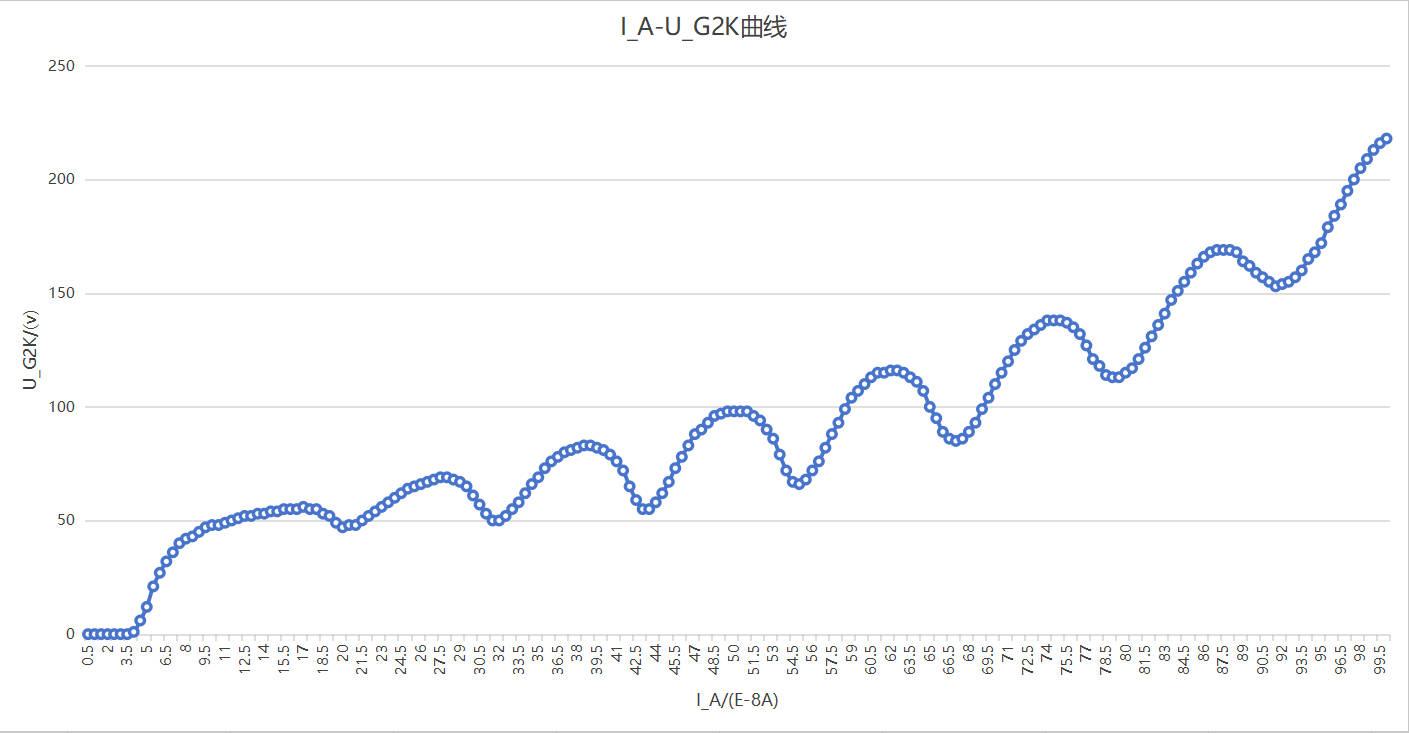
\includegraphics[width=0.8\textwidth]{手动测量曲线.jpg}
\caption{手动测量数据的$I_A$–$U_{G2K}$拟合曲线}
\label{fig:手动测量曲线}
\end{figure}
记录7个峰值对应的电压$U_{G2K}$如下表所示:
\begin{table}[htbp]
\centering
\caption{表 2-3 计算氩原子第一激发电势实验数据记录表}
\label{tab:argon_excitation_calc}
\begin{tabular}{|c|c|c|c|c|c|c|c|}
\hline
峰值序号 $n$ & 1 & 2 & 3 & 4 & 5 & 6 & 7 \\
\hline
$U_{G2K}$ (V) & 19.5 & 29.5 & 40.5 & 52.0 & 64.0 & 76.5 & 89.0 \\
\hline
\end{tabular}
\end{table}

将数据代入逐差法公式:
\begin{align*}
U_0 &= \frac{1}{4} \cdot \frac{(U_5 - U_1) + (U_6 - U_2) + (U_7 - U_3)}{3}  \\
&= \frac{1}{4}\cdot\frac{(64.0 - 19.5) + (76.5 - 29.5) + (89.0 - 40.5)}{3}
= \frac{46.6667}{4} = \SI{11.667}{\volt}
\end{align*}
理论值 $U_{\text{理}} = \SI{11.6}{\volt}$,相对误差:
\[
\delta = \left| \frac{11.667 - 11.6}{11.6} \right| \times 100\% = \SI{0.58}{\percent}
\]

由于手动与自动测量均使用同一套仪器,B类不确定度相同,仍为:
\[u(U_0)\approx \SI{0.118}{\volt}\]

最终结果:
\[
\boxed{U_0 = (\num{11.67} \pm \num{0.12})~\mathrm{V}}
\]

\subsection{误差分析(20分)}
分析知,误差主要来源于以下几个方面:
\begin{enumerate}
\item \textbf{仪器稳定性误差:} 系统预热不足会导致电子发射和原子状态不稳定,引起板极电流读数漂移;同时,环境温度波动及电源电压起伏会引入测量噪声,共同影响曲线的稳定性和峰值判读的准确性。
\item \textbf{测量方法与精度误差:} 加速电压的离散性调节导致真实峰值可能存在于记录点之间,引入插值误差;同时,人为判读峰谷位置时存在主观视差,加之仪器老化可能引起曲线特性畸变,共同构成了测量值与读数的不确定度。
\item \textbf{物理模型与系统偏差:} 电极间的接触电势差会系统性地改变电子的实际动能,使电压读数产生固定偏移;此外,理论模型忽略了氩原子的热运动,其无规则碰撞会加宽并轻微移动峰值位置,导致测量结果与理想值存在固有偏差。
\end{enumerate}
\subsection{实验探讨(10分)}
本实验通过弗兰克-赫兹管观测电子与氩原子的碰撞过程,测量其第一激发电位。实验关键在于通过自动扫描与手动测量两种模式获取$I_A-U_{G2K}$特性曲线,并采用逐差法和作图法处理电压数据,有效减小测量误差。最终获得的激发电位值与理论预测相符,直观验证了原子能级量子化的基本事实。
\section{思考题(10分)}
\subsection{探究灯丝电压$U_{F1F2}$大小对$I_A-U_{G2K}$曲线的影响}
灯丝电压决定了阴极的加热温度,进而决定了单位时间内发射出的热电子数量(即发射电流),主要影响曲线的整体幅度,而非峰值位置。
\par
当增大$U_{F1F2}$时,阴极温度升高,发射的电子流密度显著增加,导致$I_A$整体增大,曲线的峰值和谷值均上移,但峰间电压间隔保持不变。
\par
同理,减小$U_{F1F2}$会导致曲线整体下移,但即第一激发电位$U_0$的测量值基本不变。

\subsection{探究栅极电压$U_{G1K}$大小对$I_A-U_{G2K}$曲线的影响}
$U_{G1K}$是一个预加速电压,用于将电子从阴极拉出并穿过第一栅极G1,与拒斥电压$U_{G2A}$共同构成了一个筛选电子的“能量门槛”。
\par
若增大$U_{G1K}$,电子在进入主加速区(G1-G2)之前就获得了较高的初始能量,使得电子只需一个较小的$U_{G2K}$就能达到激发氩原子的临界能量$U_0$。因此,曲线的第一个峰值位置会向左移动。同时,更多的低能电子因此有足够能量到达板极,曲线起始段的电流会更大。
反之,减小$U_G1K$会使第一个峰值位置向右移动。
\par
一旦电子开始周期性获得并损失能量,后续峰谷的间距依然是原子的本征属性,基本不变。但需要注意的是,$U_{G1K}$设置不当可能导致曲线起始段畸变,影响第一个$U_0$值的准确读取。
\subsection{探究拒斥电压$U_{G2A}$大小对$I_A-U_{G2K}$曲线的影响}
$U_{G2A}$在第二栅极G2和板极A之间建立一个反向的减速电场,只有碰撞后剩余动能大于$eU_{G2A}$的电子才能克服该电场到达板极形成电流$I_A$。
\par
增大$U_{G2A}$会提高电子到达板极的能量门槛。在峰值处,电子刚刚经历非弹性碰撞,能量损失最大,本已勉强能越过门槛,现在门槛提高,它们更难以到达板极,导致峰值电流显著下降。而在谷值处,电子因能量不足无法激发原子,本身剩余能量就高,门槛提高对它们的影响相对较小。
综合效果就是,峰谷差值变小,曲线变得平坦,峰谷对比度下降,同时整体电流水平降低。
\par
同理,减小$U_{G2A}$会降低电子到达板极的门槛,使得峰值电流增加,峰谷差值增大,曲线峰形更尖锐。
\par
理论上,峰位由碰撞能量决定,与筛选条件无关,因此$U_0$不变,但在实际测量中,如果$U_{G2A}$过大,会导致峰值过于平坦而难以精确判定其位置,引入测量误差。
\end{fullreportonly}
\newpage
\insertnotes
\end{document}